\section{Background and Context}
\label{sec:background}

\begin{figure}[t!]
\begin{center}
\begin{tabular}{c}
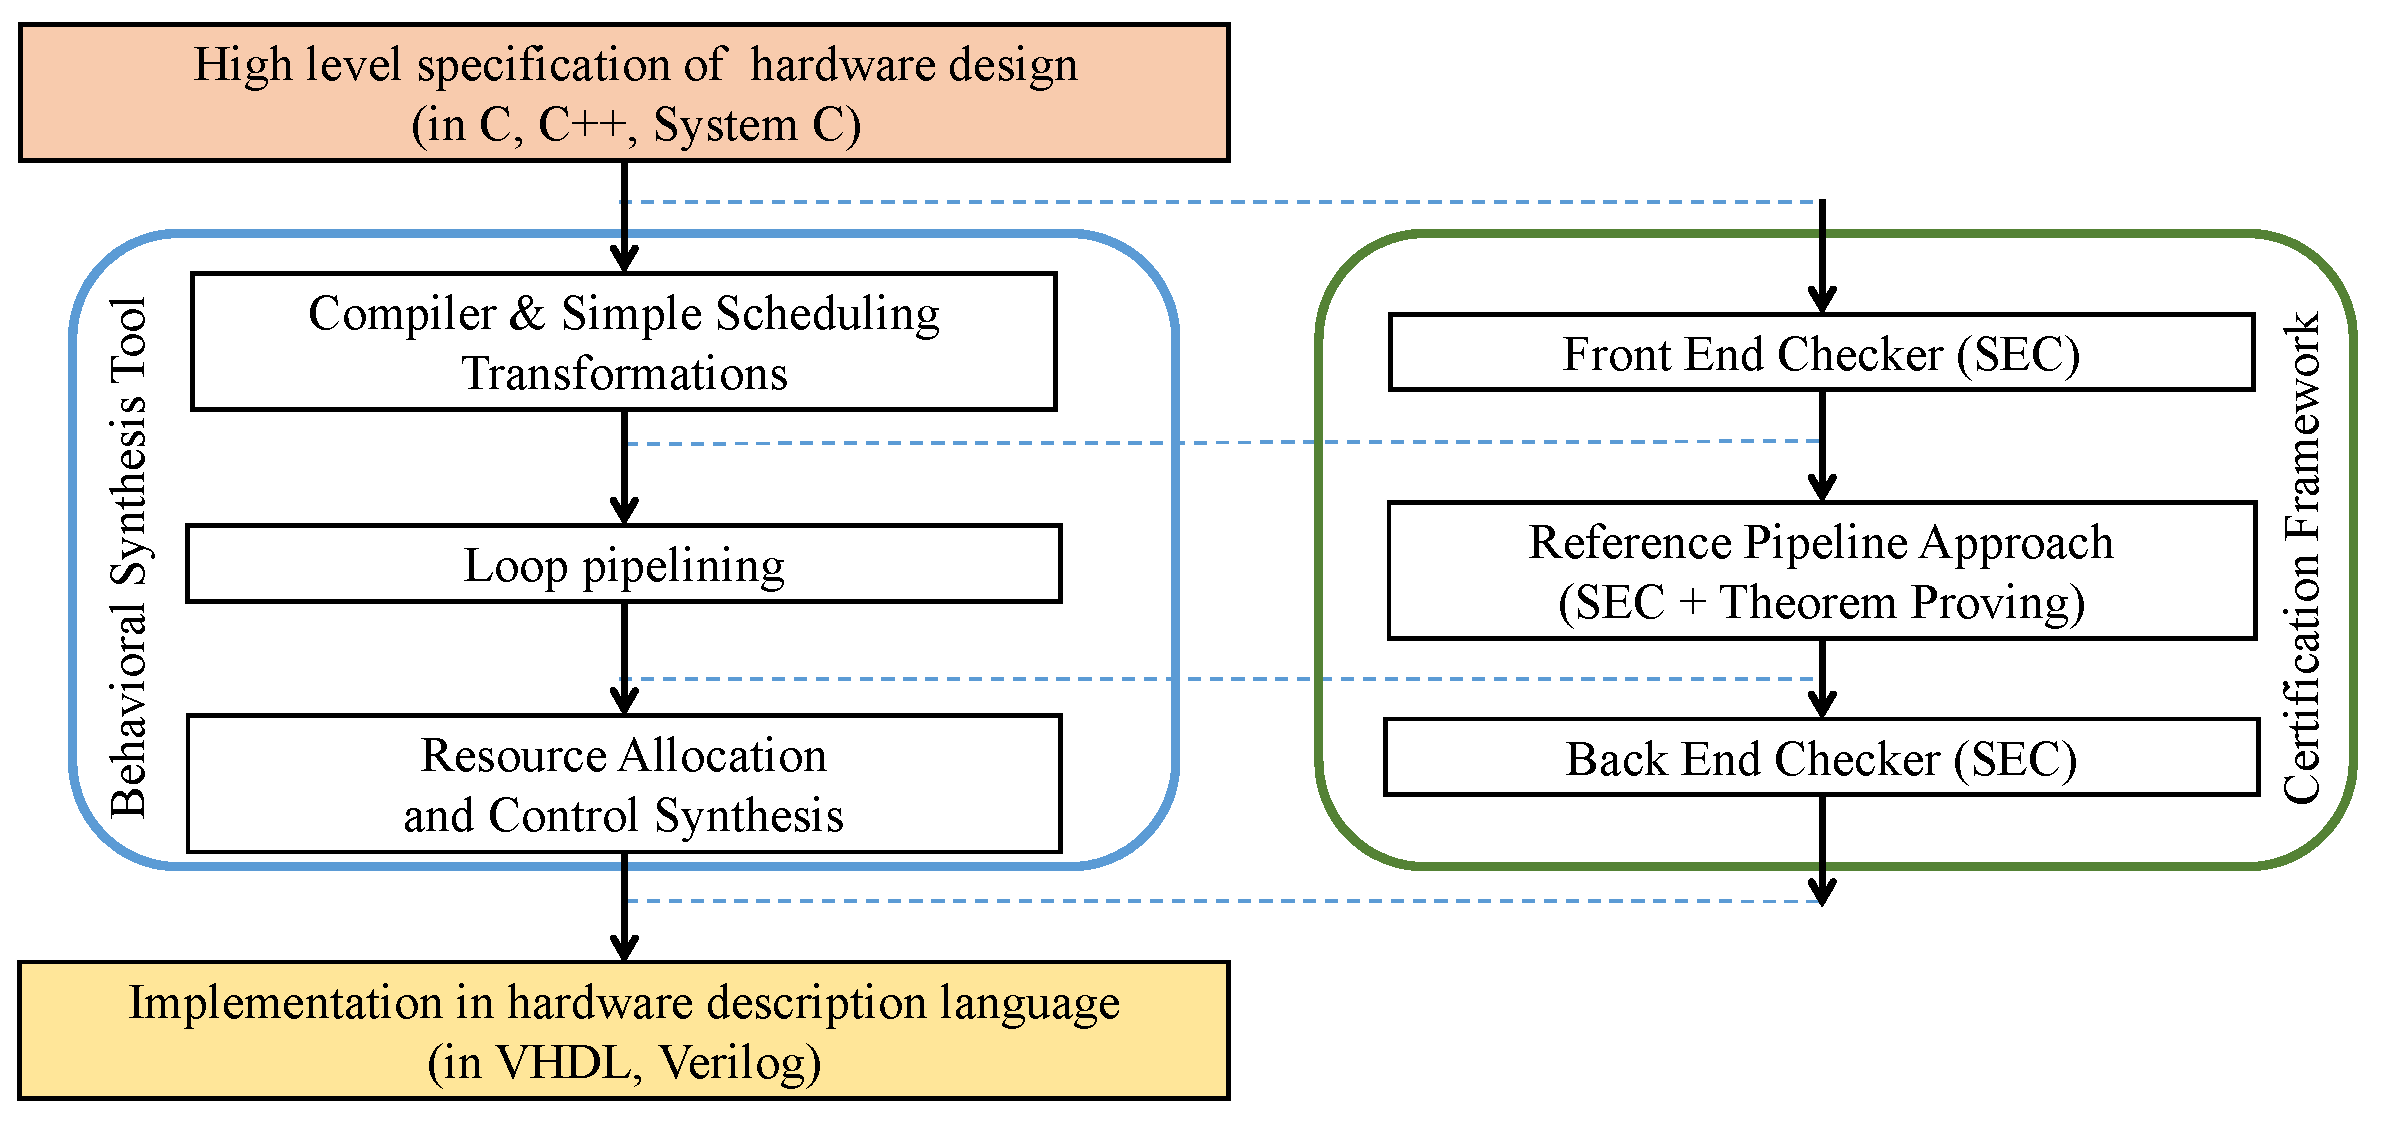
\includegraphics[height=2in]{fig-proposal/certification-framework}
\end{tabular}
\end{center}
\caption{Certification Model for Behaviorally Synthesized Pipelines}
\label{fig:certification-framework}
\end{figure}

The overall goal of the project is to provide a mechanized framework
for certifying hardware designs synthesized from ESL specifications by
commercial behavioral synthesis tools.
One obvious approach is to apply standard verification techniques (%\eg, 
SEC or
theorem proving) on the synthesized RTL itself.
Unfortunately, such a methodology is not practical.
As mentioned earlier, the large gap in abstraction
between the ESL and RTL descriptions means that there is little
correspondence in internal variables between the two.  Consequently,
direct SEC between the two reduces to cost-prohibitive computation of
input-output equivalence. On the other side, applying theorem proving
is also troublesome since extensive manual effort is necessary and
this effort needs to be replicated for each different synthesized
design. It is also infeasible to
directly certify the implementation of the {\em synthesis tool} via
theorem proving.  In addition to being highly complex and thus
potentially requiring prohibitive effort to formally verify with any
theorem prover, the implementations are typically closed-source and
closely guarded by EDA vendors and thus out of reach of external
automated reasoning communities.

To address this problem, previous work developed two key SEC
solutions, which we will refer to below as {\em Back-end} and {\em
Front-end}.  We then discuss the gap between them, which is being
filled by theorem proving efforts in this dissertation. The certfication model 
is illustrated in Figure~\ref{fig:certification-framework}.
\medskip

\noindent {\bf Back-end SEC:} The key insight behind
back-end SEC is that automated SEC techniques, while
ineffective for directly comparing synthesized RTL with the
top-level ESL description, are actually suitable to compare
the RTL with the intermediate representation (IR) generated
by the tools after the high-level (compiler and scheduling)
transformations have been applied.  In particular,
operation-to-resource mappings generated by the synthesis
tool provide the requisite correspondence between internal
variables of the IR and RTL.  Furthermore, a key insight is
that while the implementations of transformations are
unavailable for commercial EDA tools, most tools provide
these IRs after each transformation application together
with some other auxiliary information.  To exploit these, an
SEC algorithm was developed between the IR (extracted from
synthesis tool flow after these transformations) and
RTL~\cite{rhcxy:atva-09,hxry:date-10,kechengthesis,Yang2013}. 
The approach scales
to tens of thousands of lines of synthesized RTL.

\medskip

\noindent {\bf Front-end SEC:} Of course the back-end SEC
above is only meaningful if we can certify that the input
ESL indeed corresponds to the extracted IR produced after
the compiler and scheduling transformations applied in the
first two phases of synthesis. To address this, another SEC
technique was developed to compare two IRs~\cite{zhenkun:iccd-13,zhenkun2,zhenkun3}.  The idea then
is to obtain the sequence of intermediate representations
$\mbox{IR}_0,\ldots,\mbox{IR}_n$ generated by the compiler
and scheduling transformations, and compare each pair of
consecutive IRs with this new algorithm.  Then back-end SEC
can be used to compare $\mbox{IR}_n$ with the synthesized
RTL, completing the flow.

\bigskip

\noindent {\bf A Methodology Gap:} Unfortunately, the front-end SEC
algorithm can only compare two IRs that are structurally close.  If a
transformation significantly transforms the structure of an IR then
the heuristics for detecting corresponding variables between the two
IRs will not succeed, causing equivalence checking to fail.
Unfortunately, loop pipelining falls in the category of
transformations that significantly changes the structure of the IR.
It is a quintessential transformation that changes the control/data
flow and introduces additional control structures (%\eg, 
to eliminate
hazards).  This makes front-end SEC infeasible for its certification.
Furthermore, most commercial implementations are of course
proprietary and consequently not available to us for review; applying
theorem proving on those implementations is not viable from a
methodology perspective.  Thus a specialized approach is warranted for
handling its certification.


